% Provenance (never printed): see sources/outline_sources.md (Year 2: the solar nebula
% and the condensation sequence; planetesimals and embryos; chondrites, achondrites and
% irons; the age of the Solar System; differentiation of planets). Curves from
% figdata/bachelor-2/nebula.py, condensation.py, al26.py, meteorites.py; exercise and
% problem values in the Book 4 scratch calculator calc/ch02.py.
\chapter{تكوّن الكواكب والنيازك}\label{ch:b2:planet-formation-meteorites}

يدخل الغلافَ الجوي للأرض كلَّ عام نحو خمسة عشر ألف طن من غبار الفضاء؛ يحترق معظمه
أو يترسّب على هيئة كُريّات مجهرية، ومن حين إلى آخر يسقط حجر بحجم قبضة اليد مصحوبًا
بكرة نارية ودويّ اختراق جدار الصوت. ومعظم هذه الأحجار شظايا من الكويكبات، وكثير منها
لم يكد يتغيّر منذ تكوّنه. فإذا قطعنا أحدها وصقلناه ظهرت فيه حُبيبات بحجم المليمتر من
صخر كان منصهرًا، وحبيبات بيضاء غير منتظمة من معادن الكالسيوم والألومنيوم، ورقائق من
الفلز، وكلها مثبّتة في ملاط داكن دقيق الحبيبات. وتلك الحبيبات البيضاء هي أقدم المواد
الصلبة في المجموعة الشمسية: تعطيها نظائر الرصاص عمرًا قدره 4567 مليون سنة. وتؤرّخ ساعةٌ ثانية،
هي تحلّل نظير مشعّ للألومنيوم اختفى منذ زمن بعيد، المكوّناتِ الأخرى نسبةً إليها بدقة
تبلغ جزءًا من مليون سنة. يتابع هذا الفصل قرص الفصل السابق وهو يتحوّل إلى كواكب: أيّ
المواد الصلبة يتكاثف من الغاز وهو يبرد، وأين؛ وكيف ينمو الغبار إلى أجسام يبلغ قطرها
كيلومترات ثم إلى كواكب؛ وما النيازك، وكيف تؤرّخ هذه الأحداث؛ ولماذا انصهرت بعض
الأجسام الأولى وكوّنت نوى من الحديد بينما بقيت أخرى على الحال التي تكوّنت
عليها.
% ledger: rojas21:flux, lugaro:cai, gail:meteorites

\begin{recall}
تحيط بالنجوم الفتيّة أقراصٌ كوكبية أوّلية تزول في غضون بضعة ملايين من السنين؛ والحبيبة
الواقعة في ضوء نجم على البُعد $r$ منه، ولمعانه $L$، تستقرّ عند $T = \bigl(L/(16\pi\sigma r^2)\bigr)^{1/4}$
(\cref{ch:b2:ism-star-formation}). والكويكبات أجسام صغيرة صخرية أو فلزية من المجموعة
الشمسية، يدور معظمها بين المرّيخ والمشتري (مجلد السنة
الأولى). وتتحلّل النواة المشعّة باحتمال $\lambda$ في وحدة
الزمن: $N = N_0 e^{-\lambda t}$؛ وعمر النصف هو $\ln 2/\lambda$، ومتوسط
العمر $\tau = 1/\lambda$ (الفيزياء). وفي نظام مغلق تقع العيّنات المشتركة المنشأ ذات
النسب المختلفة بين الأم والوليد على مستقيم واحد، هو خط التساوي الزمني، يعطي ميلُه العمرَ
ويعطي مقطعُه النسبةَ الابتدائية (مجلد السنة الأولى).
يتطلّب تسخين كتلة $m$ سعتها الحرارية النوعية $c$ بمقدار $\Delta T$ الطاقةَ
$mc\,\Delta T$ (الفيزياء).
\end{recall}

\section{السديم الشمسي}

\begin{definition}[السديم الشمسي]\label{def:b2:planet-formation-meteorites:nebula}
\emph{السديم الشمسي}\index{السديم الشمسي} هو \omterm{def:b2:ism-star-formation:disc}{القرص الكوكبي الأوّلي} من الغاز
والغبار الذي أحاط بالشمس الفتيّة، والذي تكوّنت منه الكواكب وأقمارها
والكويكبات والمذنّبات.
\end{definition}

كم كانت كمية المادة التي حواها؟ يأتي حدٌّ أدنى من الكواكب نفسها.
فلنُضِف إلى كل كوكب ما يكفي من الهيدروجين والهيليوم ليصير تركيبه تركيب
الشمس، ولنوزّع الناتج على حلقة مركزها مداره، فنجد أن الكثافة السطحية،
أي الكتلة في وحدة المساحة من القرص، تتناقص مع البُعد عن
الشمس. ويسمّى هذا البناء \emph{السديم الشمسي ذا الكتلة
الدنيا}\index{السديم الشمسي ذو الكتلة الدنيا}. وفي صيغة شائعة الاستعمال تكون الكثافة
السطحية للغاز
\[
  \Sigma_g = \qty{2200}{g.cm^{-2}}\left(\frac{r}{\qty{1}{au}}\right)^{-3/2},
\]
وكثافة المواد الصلبة $\Sigma_p = \qty{33}{g.cm^{-2}}\,Z_{\mathrm{rel}}\,
(r/\qty{1}{au})^{-3/2}$، حيث $Z_{\mathrm{rel}}$ هو جزء المادة القابلة للتكاثف
الذي صار صلبًا فعلًا: $0.33$ حيث لم يتكاثف إلا الصخر
والفلز، ونحو $0.78$ حيث انضمّ إليهما جليد الماء، و$1$ وراء الموضع
الذي يتجمّد فيه الميثان. والأرقام غير مؤكدة: فمحتوى المشتري من العناصر الثقيلة
لا يُعرف إلا ضمن عامل أربعة، وليس من الضروري أن تكون الكواكب قد
تكوّنت حيث تدور الآن.
% ledger: cy10:mmsn

\begin{proposition}[كتلة قرص]\label{prop:b2:planet-formation-meteorites:disc-mass}
يحوي قرصٌ كثافته السطحية $\Sigma(r) = \Sigma_1 (r/r_1)^{-3/2}$، داخل
نصف القطر $R$، الكتلة
\[
  M(R) = 4\pi\Sigma_1 r_1^2 \left(\frac{R}{r_1}\right)^{1/2}.
\]
ومعظم الكتلة يقع بعيدًا: فمضاعفة نصف القطر تزيد الكتلة بنسبة \qty{41}{\percent}.
\end{proposition}

\begin{proof}
مساحة حلقة نصف قطرها $r$ وعرضها $\mathrm dr$ هي $2\pi r\,\mathrm dr$، ومنه
\[
  M(R) = \int_0^R 2\pi r\,\Sigma_1 \left(\frac{r}{r_1}\right)^{-3/2}\mathrm dr
       = 2\pi\Sigma_1 r_1^{3/2}\int_0^R r^{-1/2}\,\mathrm dr
       = 4\pi\Sigma_1 r_1^{3/2} R^{1/2},
\]
وهي الصيغة؛ والتكامل متقارب عند $r = 0$. ومضاعفة $R$
تضرب $M$ في $\sqrt 2 = 1.41$.
\end{proof}

ومع $\Sigma_1 = \qty{2.2e4}{kg.m^{-2}}$ عند $r_1 = \qty{1}{au}$، يحوي السديم ذو الكتلة
الدنيا $0.03$ كتلة شمسية داخل \qty{100}{au} (\cref{exo:b2:planet-formation-meteorites:5}). أمّا الأقراص
المرصودة حول نجوم عمرها مليون سنة، والتي تُوزن بتوهّج غبارها في الأطوال الموجية
المليمترية، فتحوي من 0.001 إلى 0.1 كتلة شمسية: فالسديم ذو الكتلة الدنيا
يقع بارتياح بينها.
% ledger: cy10:mmsn

ومعظم هذه الكتلة غاز لن يتكاثف أبدًا. فقد وُلدت الشمس
بكسر كتلي من الهيدروجين $X_0 = 0.711$، ومن الهيليوم $Y_0 = 0.274$، ومن
العناصر الأثقل كلها مجتمعةً $Z_0 = 0.0149$ فقط. وتبريد غاز بهذا
التركيب حتى يتجمّد كل ما يمكن أن يتجمّد لا يحوّل إلى مواد صلبة إلا
\qty{1.5}{\percent} من كتلته: \qty{0.49}{\percent} من الصخر
والفلز، و\qty{1.0}{\percent} من جليد الماء والميثان والأمونيا، منها
\qty{0.57}{\percent} لجليد الماء وحده. ومن هذا الجزء الصغير بُنيت الكواكب الصخرية
كلها ونوى الكواكب العملاقة.
% ledger: lodders:protosolar, lodders:condensates

تحدّد درجةُ حرارة القرص ما هو صلب وأين. فالقرص الذي لا يسخّنه إلا نجمه، أي
القرص \emph{السلبي}، دافئ عند سطحه حيث ترى الحبيبات
النجم مباشرة (القضية في \cref{ch:b2:ism-star-formation})، وأبرد كثيرًا في
مستواه الأوسط، الذي لا يتلقّى إلا الأشعة تحت الحمراء التي تعيد بثّها
حبيبات السطح تلك. ومن أجل نجم فتيّ كتلته كتلة شمسية واحدة يعطي نموذج لمثل هذا القرص
درجة حرارة المستوى الأوسط
\[
  T = \qty{120}{K}\left(\frac{r}{\qty{1}{au}}\right)^{-3/7}.
\]
وتراكم الغاز عبر القرص، الذي يحرّر طاقة جاذبية، يجعل المستوى الأوسط أسخن،
ولا سيما في البداية وقرب النجم (الشكل أدناه).
% ledger: cy10:passive

\begin{omfigure}
\begin{tikzpicture}
\begin{axis}[omrecord, width=0.82\linewidth, height=6.2cm, xmode=log, ymode=log,
  xmin=0.1, xmax=100, ymin=10, ymax=1000,
  xlabel={\foreignlanguage{arabic}{البُعد عن النجم $r$ \babelsublr{(\unit{au})}}}, ylabel={\foreignlanguage{arabic}{درجة الحرارة \babelsublr{(\unit{K})}}},
  tick label style={font=\scriptsize}, label style={font=\small},
  legend pos=north east, legend style={font=\scriptsize, draw=black!30}]
\addplot[thick, red!70!black] table[x=r_au, y=T_grain] {figdata/out/bachelor-2-nebula-temp.dat};
\addlegendentry{حبيبات في ضوء النجم المباشر}
\addplot[thick, blue!70!black] table[x=r_au, y=T_mid] {figdata/out/bachelor-2-nebula-temp.dat};
\addlegendentry{المستوى الأوسط لقرص سلبي}
\addplot[black!50, densely dashed, domain=0.1:100, samples=2] {182};
\addplot[black!50, densely dashed, domain=0.1:100, samples=2] {41};
\node[font=\scriptsize, anchor=south east] at (axis cs:95,182) {جليد الماء، \qty{182}{K}};
\node[font=\scriptsize, anchor=north west] at (axis cs:0.46,41) {جليد الميثان، \qty{41}{K}};
\draw[blue!70!black, -latex] (axis cs:0.38,25) -- (axis cs:0.38,175);
\node[font=\scriptsize, blue!70!black, anchor=north] at (axis cs:0.38,25) {\qty{0.4}{au}};
\draw[red!70!black, -latex] (axis cs:2.34,25) -- (axis cs:2.34,175);
\node[font=\scriptsize, red!70!black, anchor=north] at (axis cs:2.34,25) {\qty{2.3}{au}};
\end{axis}
\end{tikzpicture}

\par\smallskip{\small درجتا حرارة لقرص حول نجم لمعانه لمعان شمسي واحد.
بالأحمر: حبيبة سوداء في ضوء النجم المباشر (\cref{ch:b2:ism-star-formation}). بالأزرق:
المستوى الأوسط لقرص سلبي حول نجم فتيّ كتلته كتلة شمسية، محجوب عن الضوء
المباشر. جليد الماء مستقر تحت \qty{182}{K}: يحدّد السهمان الموضع الذي يقطع فيه كل منحنى
ذلك الخط. وقد وقع \omterm{def:b2:planet-formation-meteorites:snow-line}{خط الثلج} الحقيقي بين حدّين كهذين وتحرّك مع تطوّر
القرص. البيانات: تشيانغ ويودين (2010)؛ لودرز (2003).}
% ledger: cy10:passive, lodders:phases, cy10:mmsn, sun:L, const:sigma
\end{omfigure}

\section{تسلسل التكاثف}

لنتخيّل غاز السديم، قرب الشمس الفتيّة، ساخنًا بما يكفي ليكون كل
عنصر بخارًا، ولندعه يبرد ببطء يكفي لأن يبقى الغاز والمواد الصلبة
في توازن كيميائي. فمع انخفاض درجة الحرارة يغادر كل عنصر الغاز بدوره إلى
مادة صلبة، إما مركّبًا خاصًّا به وإما
ذائبًا في مادة صلبة تكوّنت من قبل.

\begin{definition}[درجة حرارة التكاثف، تسلسل التكاثف]
\label{def:b2:planet-formation-meteorites:condensation}
\emph{درجة حرارة التكاثف}\index{درجة حرارة التكاثف} لعنصر في غاز يبرد،
تركيبه وضغطه معلومان، هي درجة الحرارة
التي يكون عندها نصفه قد انتقل إلى مواد صلبة في التوازن الكيميائي (\emph{درجة
حرارة التكاثف عند 50 في المئة}؛ أمّا درجة الحرارة التي تظهر عندها أولى مواده
الصلبة فهي درجة حرارة \emph{الظهور}).
و\emph{تسلسل التكاثف}\index{تسلسل التكاثف} هو الترتيب الذي تظهر به
العناصر ومركّباتها الصلبة كلما برد الغاز.
\end{definition}

تُجرى الحسابات لغاز ذي تركيب شمسي عند ضغط كلي قدره
$10^{-4}$ بار، وهو ضغط نموذجي للسديم قرب \qty{1}{au}. وأولى المواد الصلبة
أكاسيد الألومنيوم والكالسيوم (الجدول أدناه)، التي تتكوّن عند نحو
\qty{1700}{K}؛ ويتكاثف معظم المادة المكوّنة للصخور، أي سيليكات المغنيسيوم
وفلز الحديد، قرب \qty{1350}{K}؛ وينتظر كبريتيد الحديد حتى
\qty{704}{K}، وجليد الماء حتى \qty{182}{K}.
% ledger: lodders:phases

\begin{table}[h]
\centering
\small
\begin{tabular}{lll}
\hline
المادة الصلبة & الصيغة & تظهر عند (K)\\
\hline
الكوراندوم & \ce{Al2O3} & 1677\\
الهيبونيت & \ce{CaAl12O19} & 1659\\
البيروفسكيت & \ce{CaTiO3} & 1593\\
السبينل & \ce{MgAl2O4} & 1397\\
فلز الحديد والنيكل & \ce{Fe} مع \ce{Ni} و\ce{Co} و\ce{Cr} & 1357\\
الفورستريت & \ce{Mg2SiO4} & 1354\\
الشرايبرسيت & \ce{Fe3P} & 1248\\
الترويليت & \ce{FeS} & 704\\
المغنتيت & \ce{Fe3O4} & 371\\
جليد الماء & \ce{H2O} & 182\\
هيدرات الأمونيا & \ce{NH3.H2O} & 131\\
كلاثرات الميثان & \ce{CH4.7H2O} & 78\\
\hline
\end{tabular}
\caption{\omterm{def:b2:planet-formation-meteorites:condensation}{تسلسل التكاثف} لغاز تركيبه تركيب المجموعة الشمسية عند
$10^{-4}$ بار: درجة الحرارة التي تظهر عندها كل مادة صلبة أوّل مرة. يدخل الصوديوم
والبوتاسيوم في الفلسبار؛ ويذوب النيكل والكوبالت والكروم في الفلز.
البيانات: لودرز (2003).}
\label{tab:b2:planet-formation-meteorites:sequence}
% ledger: lodders:phases
\end{table}

تفرز درجاتُ حرارة التكاثف عند 50 في المئة العناصرَ في مجموعات حسب
تطايرها (الشكل أدناه). فالعناصر التي تتكاثف فوق المغنيسيوم والسيليكون
والحديد \emph{عصيّة على التبخّر}؛ والتي تتكاثف تحتها \emph{متطايرة}.
ويقسّم لودرز كل جانب تقسيمًا أدقّ: فالعناصر فائقة العصيان، فوق
\qty{1650}{K}، تشمل الألومنيوم والزركونيوم والعناصر الأرضية النادرة الثقيلة
والفلزات الأوزميوم والرينيوم والتنغستن؛ والعناصر شديدة العصيان
(\qtyrange{1500}{1650}{K}) تشمل الكالسيوم والتيتانيوم؛ والعناصر العصيّة
(\qtyrange{1360}{1500}{K}) تشمل السترونشيوم والباريوم والفاناديوم والبلاتين؛
والعناصر
\emph{الشائعة}، المغنيسيوم والسيليكون والحديد، تتكاثف بين \num{1290}
و\qty{1360}{K}، ومعها النيكل والكوبالت والكروم؛ والعناصر المتوسطة
التطاير، ومنها الصوديوم والبوتاسيوم والفوسفور والنحاس والزنك
والرصاص، تتكاثف بين \qty{1290}{K} وظهور الترويليت عند
\qty{704}{K}؛ والعناصر المتطايرة، ومنها الكبريت والكادميوم والثاليوم،
بين \num{704} و\qty{371}{K}؛ والعناصر شديدة التطاير، الكربون
والنيتروجين والأكسجين في صورة جليد والغازات النبيلة والزئبق، تحت ذلك.
% ledger: lodders:groups, lodders:tc-table, lodders:tc-more

\begin{omfigure}
\begin{tikzpicture}
\begin{axis}[width=0.86\linewidth, height=10.5cm, xbar, bar width=4.2pt, bar shift=0pt,
  xmin=0, xmax=1950, ymin=0.3, ymax=36.7,
  ytick={1,...,36}, yticklabels from table={figdata/out/bachelor-2-condensation-labels.dat}{name},
  y tick label style={font=\tiny}, tick label style={font=\scriptsize}, label style={font=\small},
  xlabel={\foreignlanguage{arabic}{درجة حرارة التكاثف عند 50 في المئة تحت $10^{-4}$ بار \babelsublr{(\unit{K})}}},
  xmajorgrids, grid style={black!12}, legend pos=south east, legend cell align=left,
  legend style={font=\scriptsize, draw=black!30}]
\addplot[fill=red!70!black, draw=none] table[x=T, y=idx] {figdata/out/bachelor-2-condensation-ultra.dat};
\addlegendentry{فائقة العصيان}
\addplot[fill=red!45, draw=none] table[x=T, y=idx] {figdata/out/bachelor-2-condensation-high.dat};
\addlegendentry{شديدة العصيان}
\addplot[fill=orange!60, draw=none] table[x=T, y=idx] {figdata/out/bachelor-2-condensation-refr.dat};
\addlegendentry{عصيّة}
\addplot[fill=black!55, draw=none] table[x=T, y=idx] {figdata/out/bachelor-2-condensation-common.dat};
\addlegendentry{\foreignlanguage{arabic}{شائعة (Mg وSi وFe)}}
\addplot[fill=teal!55, draw=none] table[x=T, y=idx] {figdata/out/bachelor-2-condensation-modvol.dat};
\addlegendentry{متوسطة التطاير}
\addplot[fill=blue!45, draw=none] table[x=T, y=idx] {figdata/out/bachelor-2-condensation-vol.dat};
\addlegendentry{متطايرة}
\addplot[fill=blue!20, draw=none] table[x=T, y=idx] {figdata/out/bachelor-2-condensation-hivol.dat};
\addlegendentry{شديدة التطاير}
\end{axis}
\end{tikzpicture}

\par\smallskip{\small درجات حرارة التكاثف عند 50 في المئة لعناصر عددها 36 في
غاز تركيبه تركيب المجموعة الشمسية عند $10^{-4}$ بار، ملوّنة حسب مجموعات التطاير
عند لودرز (الأكسجين: في صورة جليد الماء؛ الكربون: في صورة كلاثرات الميثان وجليد). البيانات:
لودرز (2003).}
% ledger: lodders:tc-table, lodders:tc-more, lodders:groups
\end{omfigure}

يفسّر هذا التسلسل نمطًا يسري في المجموعة الشمسية كلها. فأقدم
المواد الصلبة في النيازك مصنوعة من أولى المتكاثفات؛ والأرض والكواكب
الصخرية الأخرى فقيرة بالعناصر المتطايرة؛ وأطراف القرص البعيدة، الباردة بما يكفي
لحفظ الجليد، صنعت أجسامًا جليدية. وأهم الحدود هو حدّ الماء، لأن جليد الماء
أوفر المواد الصلبة كلها: ففي غاز ذي تركيب شمسي يوجد من جليد الماء، كتلةً، ما يعادل
الصخر والفلز معًا تقريبًا، بل أكثر منهما بعامل \num{1.17}.
% ledger: lodders:condensates

\begin{definition}[خط الثلج]\label{def:b2:planet-formation-meteorites:snow-line}
\emph{خط الثلج}\index{خط الثلج} لقرص كوكبي أوّلي هو البُعد
عن النجم الذي يصير وراءه المستوى الأوسط باردًا بما يكفي لاستقرار جليد الماء،
أي نحو \qty{180}{K} عند ضغوط القرص.
\end{definition}

\begin{proposition}[خط الثلج في قرص سلبي]
\label{prop:b2:planet-formation-meteorites:snow-line}
إذا تناقصت درجة حرارة المستوى الأوسط وفق $T = T_1 (r/r_1)^{-3/7}$، فإن خط ثلج
الماء، الذي يتكاثف عند $T_w$، يقع عند
\[
  r_s = r_1 \left(\frac{T_1}{T_w}\right)^{7/3},
\]
ووراءه تقفز الكثافة السطحية للمواد الصلبة بعامل $1 + m_w/m_r$،
حيث $m_w$ و$m_r$ كتلتا جليد الماء والصخر في الغاز.
\end{proposition}

\begin{proof}
بحلّ $T_w = T_1 (r_s/r_1)^{-3/7}$ بالنسبة إلى $r_s$ نحصل على
$r_s/r_1 = (T_1/T_w)^{7/3}$. وداخل $r_s$ لا يكون صلبًا إلا الصخر والفلز؛ ووراءه
يضيف جليد الماء كتلته $m_w$ إلى صخر $m_r$ الغاز نفسه، فتُضرب
الكتلة الصلبة في $(m_r + m_w)/m_r$.
\end{proof}

في القرص السلبي أعلاه، تعطي $T_1 = \qty{120}{K}$ و$T_w = \qty{182}{K}$
$r_s = \qty{0.38}{au}$؛ أمّا الميثان، عند \qty{41}{K}، فيتجمّد وراء \qty{12}{au}
(\cref{exo:b2:planet-formation-meteorites:6}). ومع \qty{0.57}{\percent} من جليد الماء و\qty{0.49}{\percent}
من الصخر تقفز المواد الصلبة بعامل $1 + 0.571/0.489 = 2.2$. ويضع
النموذج \omterm{def:b2:planet-formation-meteorites:snow-line}{خط الثلج} داخل مدار الأرض بكثير، وهذا لا يُظهر إلا أن
القرص الفتيّ لم يكن سلبيًا: فبتسخينه بالتراكم كان مستواه الأوسط الداخلي أدفأ،
ووقع \omterm{def:b2:planet-formation-meteorites:snow-line}{خط الثلج} أبعد، ثم تحرّك نحو الداخل مع ترقّق القرص. ووراءه
كان لدى الكواكب أكثر من ضعف المادة الصلبة لتُبنى منها، وهذا، أكثر من أي شيء آخر،
ما يفصل الكواكب الصخرية الصغيرة عن
العملاقة.
% ledger: cy10:passive, lodders:condensates

\section{من الغبار إلى الكواكب}

بين حبيبات \omterm{def:b2:ism-star-formation:ism}{الوسط بين النجمي} الميكرومترية وكواكب يبلغ قطرها آلاف
الكيلومترات نحو ثلاث عشرة رتبة من رتب الحجم. ويحسن وصف النموّ
على ثلاث مراحل. فتحت نحو سنتيمتر تلتصق الحبيبات التي تتصادم
برفق، مشدودةً بروابط كيميائية وبقوى فان دير فالس، فتبني تجمّعات
منتفشة. وفوق الكيلومتر بكثير تتماسك الأجسام بجاذبيتها الذاتية،
وتسقط شظايا التصادم عائدةً على الجسم الأكبر. وبين الاثنتين
تقع أصعب المراحل: فالأجسام من السنتيمترات إلى الأمتار أكبر من أن تلتصق
وأصغر من أن يجذب بعضها بعضًا، ويجرّها الغاز نحو الداخل. وفي
المحاكاة العددية تتجمّع مواد صلبة يبلغ قطرها من 10 إلى \qty{100}{cm} في أسراب
كثيفة تنهار تحت ثقلها مباشرة إلى أجسام يبلغ قطرها كيلومترات،
متخطّيةً الأحجام العسيرة؛ أمّا كيف عبرت المجموعة الشمسية هذه المرحلة
فلا يزال موضع نقاش.
% ledger: cy10:growth

\begin{definition}[الكويكب البدائي، الجنين الكوكبي]
\label{def:b2:planet-formation-meteorites:planetesimal}
\emph{الكويكب البدائي}\index{الكويكب البدائي} جسم صلب في قرص كوكبي أوّلي
كبير بما يكفي، من نحو كيلومتر إلى بضع مئات من الكيلومترات قطرًا،
لكي تحكم الجاذبيةُ نموَّه لا الالتصاق. و\emph{الجنين
الكوكبي}\index{الجنين الكوكبي} جسم نما، بمراكمة
الكويكبات البدائية، بما يكفي ليسود منطقته من القرص
ويكنسها من الكويكبات البدائية.
\end{definition}
% ledger: lugaro:cai

وما إن تسود الجاذبية حتى يجمح النموّ: فالجسم الأكبر قليلًا من
جيرانه يجذب \omterm{def:b2:planet-formation-meteorites:planetesimal}{الكويكبات البدائية} نحوه من مسافات أبعد، فينمو أسرع
منها، ويتقدّم عليها. ولا يتباطأ نموّه إلا حين يكون قد كنس
المواد الصلبة التي في متناوله. ثم يسود كل جنين حلقته من القرص،
وتتقاسم أجنّة كثيرة منطقة الكواكب الصخرية.

\begin{proposition}[كتلة العزلة]\label{prop:b2:planet-formation-meteorites:isolation}
يجذب جنينٌ كتلته $M$ على البُعد $r$ من نجم كتلته $M_*$
المواد الصلبة لحلقة نصف عرضها بضعة أضعاف نصف قطر هيل الخاص به
$R_H = r\,(M/3M_*)^{1/3}$. فإذا جمع كل المواد الصلبة لحلقة عرضها الكلي
$bR_H$ وكثافتها السطحية $\Sigma_p$، توقّف عن النموّ عند
\emph{كتلة العزلة}
\[
  M_{\mathrm{iso}} = \frac{(2\pi b\, r^2 \Sigma_p)^{3/2}}{(3M_*)^{1/2}} .
\]
\end{proposition}

\begin{proof}
تحوي الحلقة التي نصف قطرها $r$ وعرضها $bR_H$ الكتلة
$2\pi r\, bR_H\,\Sigma_p$. ويكون الجنين قد ابتلعها حين
$M = 2\pi b r\Sigma_p\, r\,(M/3M_*)^{1/3}$، أي
$M^{2/3} = 2\pi b r^2\Sigma_p/(3M_*)^{1/3}$؛ ورفع الطرفين إلى القوة
$3/2$ يعطي الصيغة.
\end{proof}

تأخذ النماذج $b \approx 5$. وفي السديم ذي الكتلة الدنيا تبلغ كتلة العزلة
نحو \num{0.05} كتلة أرضية عند \qty{1}{au}، بين كتلتي
القمر (\num{0.012}) والمرّيخ (\num{0.11}): فكانت أجنّة المجموعة الشمسية الداخلية
أجسامًا بهذا الحجم، واحتاجت الأرض إلى كثير منها. ووراء \omterm{def:b2:planet-formation-meteorites:snow-line}{خط الثلج}، عند \qty{5.2}{au}، تعطي المواد الصلبة الغنية بالجليد نحو
\num{0.8} كتلة أرضية، ويعطي قرصٌ فيه من المواد الصلبة \num{3.5} أضعاف الكتلة الدنيا
نحو خمس كتل أرضية (\cref{exo:b2:planet-formation-meteorites:7}): وهذا يكفي، في نماذج نموّ
المشتري، لكي تجذب نواةٌ غلافها الغازي في غضون ثلاثة ملايين سنة. وكان على
الكواكب العملاقة أن تتكوّن قبل زوال غاز القرص، في غضون بضعة
ملايين من السنين؛ وأورانوس ونبتون مكوّنان من الصخر والجليد بنسبة \qtyrange{80}{90}{\percent}
كتلةً: فلم يجمعا إلا قليلًا من الغاز.
% ledger: cy10:isolation, cy10:mmsn, earth:mass, haisch:disc-lifetime, planet:Moon.mass, planet:Mars.mass

كانت المرحلة الأخيرة من تكوّن الكواكب الصخرية عنيفة. فبعد زوال الغاز
تقاطعت مدارات الأجنّة، واندمجت في تصادمات عملاقة؛ ويُعتقد أن القمر
تكوّن من حطام أحدها، الذي ضرب الأرض
الفتيّة. ويلخّص الشكل أدناه هذا التسلسل.

\begin{omfigure}
\begin{tikzpicture}[x=1cm, y=1cm, font=\scriptsize]
\foreach \x/\t/\s in {0/{حبيبات غبار}/{\qty{1}{\micro m}},
  2.9/{تجمّعات،\\حصيّات}/{\foreignlanguage{arabic}{من \unit{mm} إلى \qty{1}{m}}},
  5.8/{كويكبات بدائية}/{\qtyrange{1}{200}{km}},
  8.7/{أجنّة\\كوكبية}/{من القمر إلى المرّيخ},
  11.6/{كواكب}/{} } {
  \node[align=center, anchor=north] at (\x,-0.9) {\t};
  \node[align=center, anchor=north, black!60] at (\x,-1.55) {\s};
}
\foreach \i in {0,...,11} {\fill[black!45] ({-0.4+0.07*mod(\i*7,11)},{-0.35+0.06*mod(\i*5,11)}) circle (0.025);}
\fill[black!35] (2.7,0.05) circle (0.12); \fill[black!45] (3.05,-0.25) circle (0.09);
\fill[black!40] (2.85,-0.45) circle (0.06); \fill[black!30] (3.15,0.15) circle (0.07);
\fill[brown!55!black!70] (5.55,0) circle (0.2); \fill[brown!50!black!60] (6.1,-0.15) circle (0.16);
\fill[brown!45!black!70] (5.85,0.32) circle (0.11);
\fill[brown!60!black!80] (8.7,-0.05) circle (0.38); \fill[brown!50!black!60] (9.25,0.35) circle (0.16);
\shade[ball color=blue!45!brown!60] (11.6,-0.05) circle (0.62);
\foreach \x in {1.2,4.1,7.0,9.95} {\draw[-latex, black!60] (\x,-0.1) -- +(0.55,0);}
\node[align=center, anchor=south, black!70] at (1.45,0.55) {التصاق};
\node[align=center, anchor=south, black!70] at (4.35,0.55) {انهيار\\الأسراب الكثيفة};
\node[align=center, anchor=south, black!70] at (7.25,0.55) {نموّ\\جامح};
\node[align=center, anchor=south, black!70] at (10.2,0.55) {تصادمات\\عملاقة};
\end{tikzpicture}

\par\smallskip{\small من الغبار إلى الكواكب في منطقة الكواكب الصخرية
(رسم تخطيطي، ليس بمقياس رسم). تلتصق الحبيبات في تجمّعات؛ وتنهار أسراب الحصيّات
إلى \omterm{def:b2:planet-formation-meteorites:planetesimal}{كويكبات بدائية}؛ وتجعل الجاذبية بعض \omterm{def:b2:planet-formation-meteorites:planetesimal}{الكويكبات البدائية} تجمح نموًّا إلى أجنّة،
تنتهي بالاندماج في كواكب. ووراء \omterm{def:b2:planet-formation-meteorites:snow-line}{خط الثلج} نمت الأجنّة أكبر واستطاعت
أسر الغاز. الأحجام من تشيانغ ويودين (2010) ولوغارو وآخرين (2018).}
% ledger: cy10:growth, lugaro:cai
\end{omfigure}

لم تحتفظ الكواكب إلا بذاكرة ضئيلة من هذا التاريخ: فقد انصهرت واختلطت وأعادت
تشكيل مادتها. والسجلّ محفوظ في الأجسام التي توقّف نموّها، أي
الكويكبات، وفي القطع التي تصل منها إلى الأرض.

\section{النيازك}

\begin{definition}[النيزك، السقطة النيزكية، اللقية النيزكية]
\label{def:b2:planet-formation-meteorites:fall-find}
\emph{النيزك}\index{النيزك} جسم صلب طبيعي آتٍ من الفضاء
نجا من عبوره الغلاف الجوي وبلغ الأرض. و\emph{السقطة
النيزكية}\index{السقطة النيزكية} نيزك جُمع بعد أن رُصد
وصوله، عادةً على هيئة كرة نارية؛ و\emph{اللقية
النيزكية}\index{اللقية النيزكية} نيزك تُعرّف عليه على الأرض دون أن يكون
سقوطه قد شوهد.
\end{definition}

تكنس الأرض من الغبار أكثر بكثير مما تكنس من الأحجار. فبالقياس في ثلج
هضبة القارة القطبية الجنوبية، يبلغ الأرضَ كل عام نحو \qty{5200}{t} من الغبار
الآتي من خارج الأرض على هيئة نيازك دقيقة وكُريّات منصهرة، من أصل نحو
\qty{15000}{t} تدخل الغلاف الجوي، يأتي معظمها من المذنّبات ونحو
خُمسها من الكويكبات. أمّا النيازك، أي الأحجار والحديديات الكبيرة بما يكفي ليُتعرّف
عليها واحدًا واحدًا، فأقل عددًا: إذ يضمّ الفهرس العالمي نحو
\num{45000} منها، ليس منها إلا \num{1107} سقطة.
% ledger: rojas21:flux, data:b4-meteorites

ولهذا التمييز أهميته. فالسقطة تُجمع في غضون أيام، قبل أن يغيّرها المطر
والأكسجين، ويُجمع كل نوع من النيازك التي تسقط على
السواء؛ أمّا اللقية فقد تكون بقيت على الأرض آلاف السنين، وتتوقّف
فرصة العثور عليها على مظهرها وعلى موضع سقوطها. وقد عُثر على نصف
اللقيات كلها في القارة القطبية الجنوبية (الإطار أدناه)، حيث البحث
منهجي. والسقطات هي العيّنة الأعدل لما يصل (الشكل أدناه):
فأكثر من أربع من كل خمس منها كوندريتات، وثلاث من كل أربع كوندريتات عادية.
% ledger: data:b4-meteorites

\begin{omfigure}
\begin{tikzpicture}
\begin{axis}[width=0.86\linewidth, height=6.3cm, ybar, bar width=7pt,
  xmin=0.4, xmax=9.6, ymin=0.1, ymax=200, ymode=log, log origin=infty,
  xtick={1,...,9}, xticklabels={عادية, كربونية, إنستاتيتية, كوندريتات أخرى,
    HED, أكوندريتات أخرى, حديدية, حجرية حديدية, غير مصنّفة},
  x tick label style={font=\scriptsize, rotate=30, anchor=north east, inner sep=1pt},
  tick label style={font=\scriptsize}, label style={font=\small},
  ylabel={\foreignlanguage{arabic}{الحصّة من العيّنة \babelsublr{(\%)}}}, legend pos=north east, xtick pos=bottom,
  legend style={font=\scriptsize, draw=black!30}, ymajorgrids, grid style={black!12}]
\addplot[fill=orange!70, draw=none] table[x=idx, y=falls_pct] {figdata/out/bachelor-2-meteorites-frac.dat};
\addlegendentry{سقطات (\num{1107})}
\addplot[fill=blue!45, draw=none] table[x=idx, y=finds_pct] {figdata/out/bachelor-2-meteorites-frac.dat};
\addlegendentry{لقيات (\num{44534})}
\end{axis}
\end{tikzpicture}

\par\smallskip{\small النيازك حسب الصنف، نسبةً مئوية من السقطات ومن
اللقيات (مقياس لوغاريتمي)؛ HED: الهواردايت واليوكرايت والديوجينايت. البيانات: نسخة
ناسا المصدَّرة من قاعدة بيانات النشرة النيزكية للجمعية النيزكية
(\num{45641} نيزكًا صالحًا).}
% ledger: data:b4-meteorites
\end{omfigure}

\begin{inthefield}[البحث عن النيازك على الجليد الأزرق]
\begin{minipage}[t]{0.6\linewidth}\vspace{0pt}
معظم الغطاء الجليدي للقارة القطبية الجنوبية ثلج أبيض، لكن على نحو
\qty{1}{\percent} من سطحه، حيث تعترض الجبال جريان الجليد،
يُفقد نحو \qty{5}{cm} من الجليد كل عام فيظهر جليد أزرق عارٍ. فالنيازك
التي سقطت على الثلج في أعلى المجرى، على مدى عشرات آلاف السنين، تُدفن،
وتُحمل مع الجليد، وتعود إلى السطح حيث يذوب ويتبخّر:
فالجليد الأزرق مصيدة. ومنذ أن بدأ الجمع المنهجي في منتصف سبعينيات القرن العشرين،
استعادت الفرق أكثر من \num{30000} عيّنة من مثل هذه الحقول، وفي
الفهرس يأتي نصف اللقيات كلها من جنوب \ang{60}\,ج. ويعبر الباحثون
الجليد في صفوف، سيرًا على الأقدام أو على عربات الثلج، ويُجمع كل حجر يُعثر عليه
مهما بدا عاديًا، كي لا تنحاز المجموعة
إلى الأحجار اللافتة. وتُصوَّر كل لقية حيث هي، لتسجيل
سياقها، وتُعطى رقمًا ميدانيًا؛ ثم تتلقّى لاحقًا اسمها الرسمي، وهو
رمز من ثلاثة أحرف لحقل الجليد يليه عام الموسم ورقم
متسلسل. وفي مختبر الحفظ تُكسر الأحجار بأدوات من
الفولاذ المقاوم للصدأ أو تُقطع جافةً بمنشار شريطي؛ أمّا الكوندريتات الكربونية،
التي قد تحوي مركّبات عضوية، فلها خزانة خاصة بها منذ عام 1978.
\end{minipage}\hfill
\begin{minipage}[t]{0.37\linewidth}\vspace{0pt}
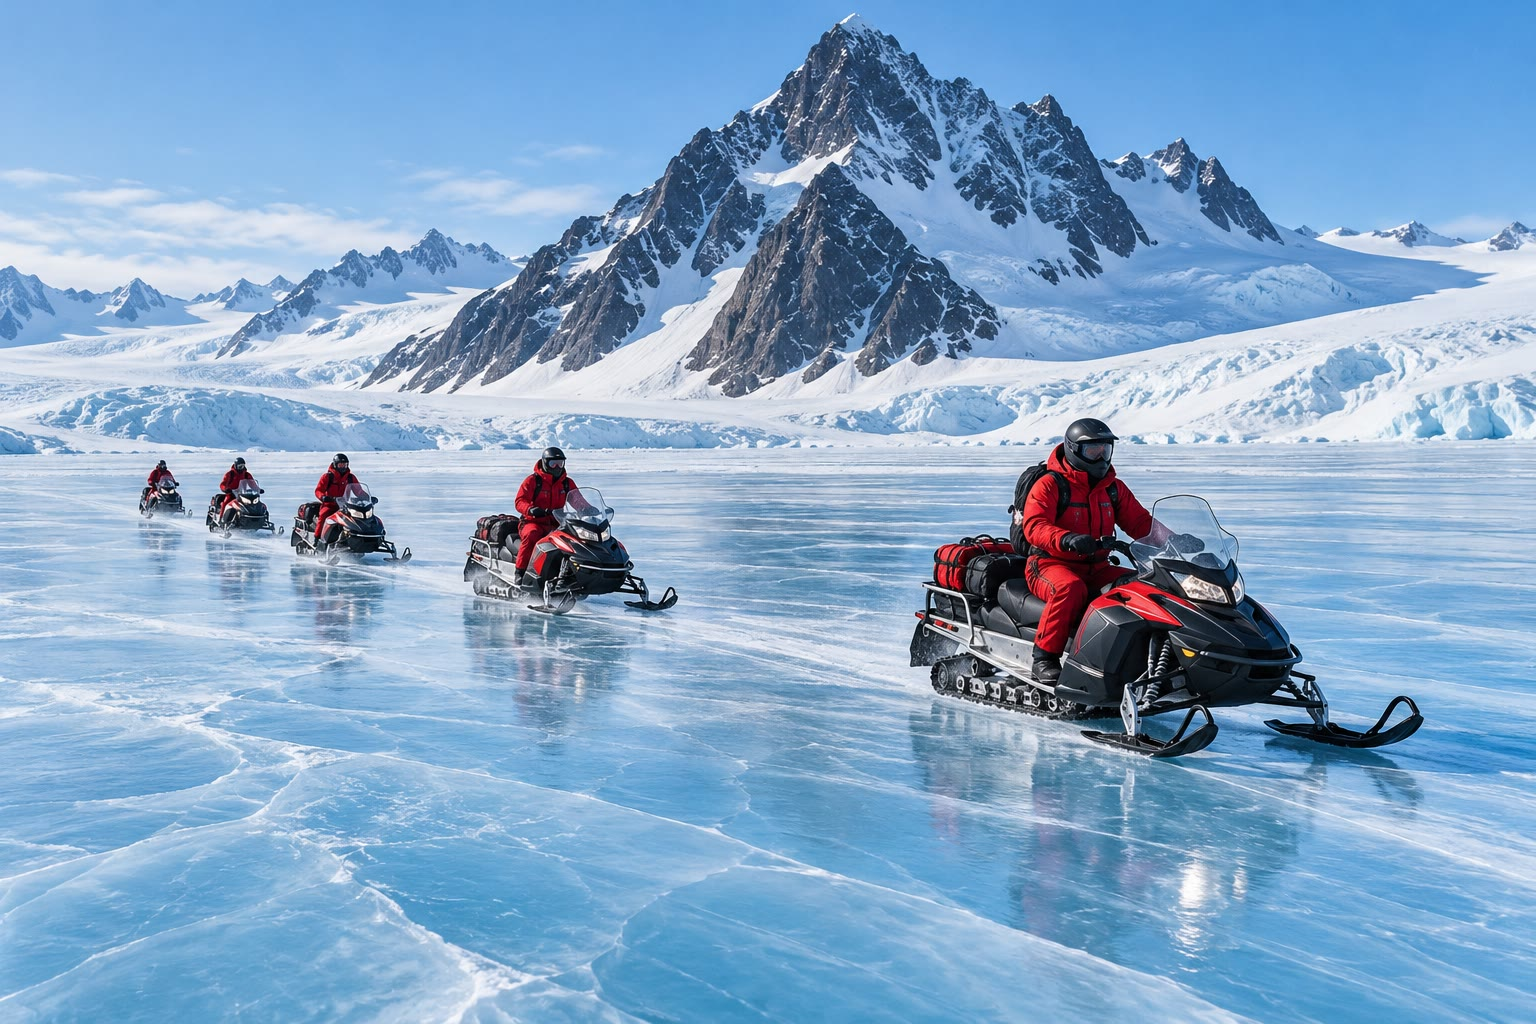
\includegraphics[width=\linewidth]{images/book4/ai/b2-blue-ice-search.jpg}

{\scriptsize صفّ من الباحثين على عربات الثلج يعبر حقلًا من الجليد الأزرق أسفل
قمة صخرية (رسم توضيحي مولَّد بالذكاء الاصطناعي).}
\end{minipage}
% ledger: folco06:blue-ice, data:b4-meteorites, nasa:antmet
\end{inthefield}

\subsection{الكوندريتات}

\begin{definition}[الكوندريت، الكوندريت الكربوني، الكوندرول، CAI]
\label{def:b2:planet-formation-meteorites:chondrule}
\emph{الكوندريت}\index{الكوندريت} نيزك حجري لم ينصهر قطّ
بعد تجمّعه، وتركيبه، باستثناء العناصر الأشد تطايرًا، قريب من تركيب
الشمس. ويتكوّن معظمه من
\emph{الكوندرولات}\index{الكوندرول}، وهي قُطيرات مستديرة، يتراوح قطرها بين عُشر المليمتر
ونحو سنتيمتر، من صخر سيليكاتي تصلّب من مصهور، مثبّتة في
أرضية دقيقة الحبيبات فيها حبيبات من فلز الحديد والنيكل ومن كبريتيد الحديد. وتحوي بعض
الكوندريتات \emph{دخائل غنية بالكالسيوم والألومنيوم}\index{الدخيلة الغنية بالكالسيوم والألومنيوم}
(CAI)، وهي حبيبات بيضاء غير منتظمة من معادن الكالسيوم والألومنيوم
والتيتانيوم، وهي أولى متكاثفات السديم. و\emph{الكوندريت
الكربوني}\index{الكوندريت الكربوني} كوندريت غني
بالكربون وبالمعادن الحاملة للماء وبالأرضية، ومحتواه من العناصر المتطايرة
هو الأقرب إلى محتوى الشمس.
\end{definition}

لم تبقَ \omterm{def:b2:planet-formation-meteorites:chondrule}{الكوندرولات} منصهرة إلا دقائق، وبردت على مدى ساعات إلى
أيام: فقد صهر تسخينٌ وميضيّ قصير محلّي في السديم، لا يزال سببه
مجهولًا، كتلًا من الغبار تجمّدت قُطيراتٍ قبل أن تُكنس
مع الغبار والفلز في \omterm{def:b2:planet-formation-meteorites:planetesimal}{كويكب بدائي}. وهي تملأ ما يصل إلى \qty{90}{\percent} من حجم أكثر
النيازك بدائيةً. وتمثّل الدخائل CAI من أقل من \qty{1}{\percent} من
الكوندريتات العادية إلى أكثر من \qty{10}{\percent} من بعض الكوندريتات الكربونية، وقد
تكوّنت في غضون نحو مئة ألف سنة بعضها من بعض.
% ledger: gail:meteorites, cy10:growth, cy10:chondrules, gail:chondrite-table, lugaro:cai

\begin{omfigure}
\begin{minipage}[c]{0.5\linewidth}
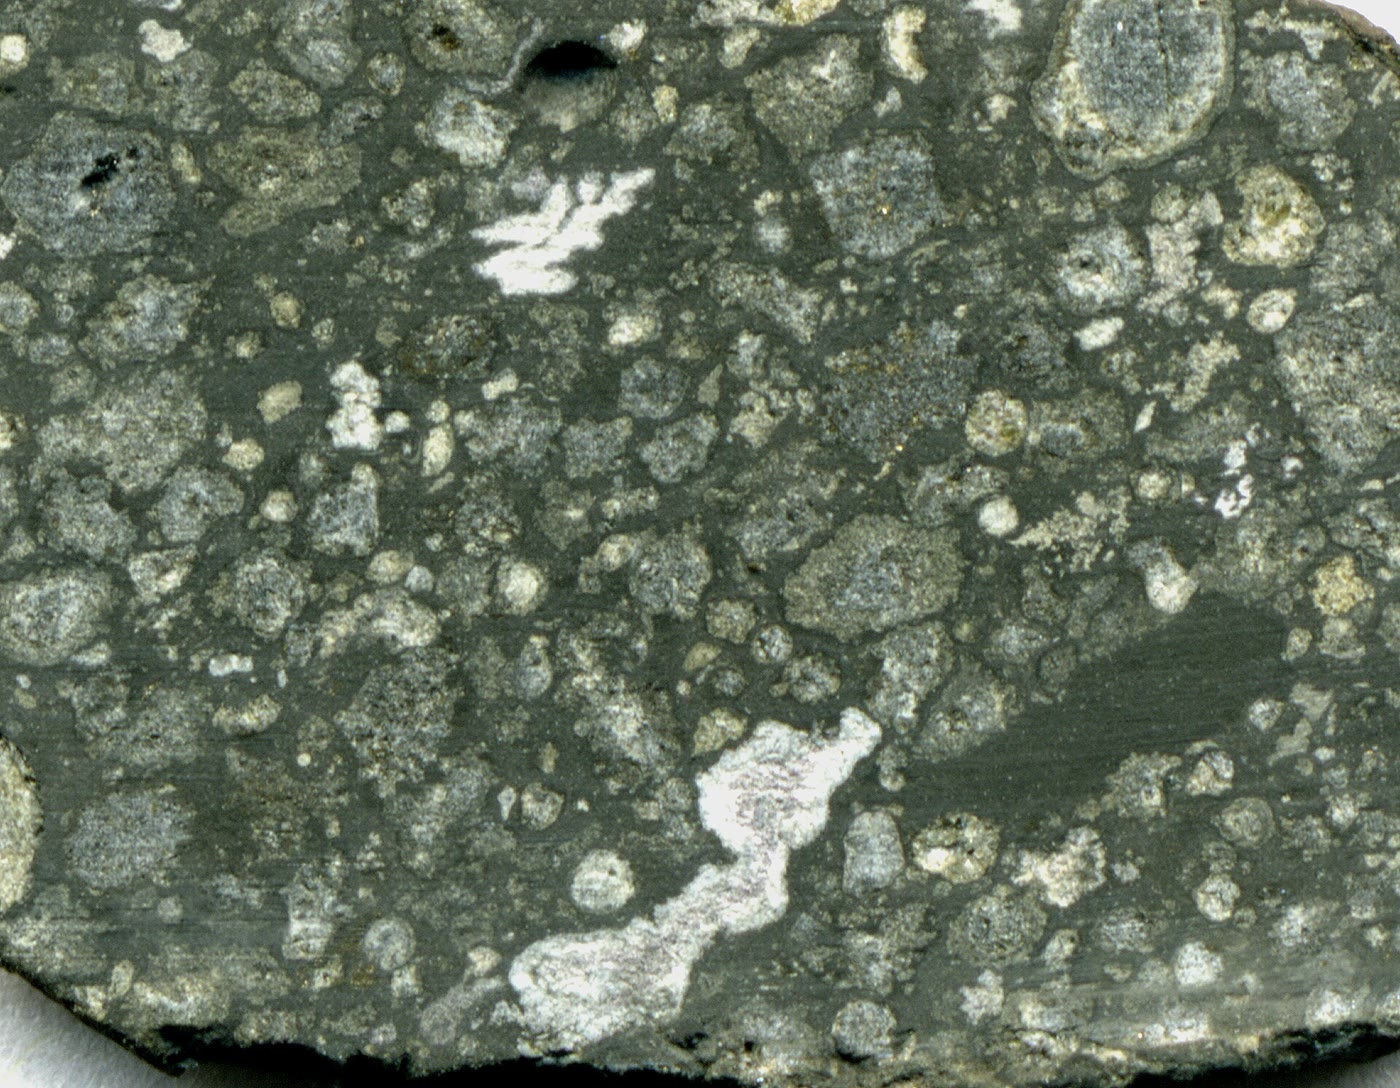
\includegraphics[width=\linewidth]{images/book4/b2-allende-chondrite.jpg}
\end{minipage}\hfill
\begin{minipage}[c]{0.46\linewidth}
{\small وجه مقطوع من كوندريت أليندي الكربوني (الصنف CV3)، الذي سقط في
شمال المكسيك عام 1969: جُمع منه نحو طنّين. الحبيبات الرمادية المستديرة
كوندرولات؛ والبقع البيضاء غير المنتظمة دخائل CAI؛ والملاط الداكن هو الأرضية. وعرض
الحقل بضعة سنتيمترات. James St.\ John, CC BY 2.0.}
\end{minipage}
% ledger: data:b4-meteorites, gail:chondrite-table
\end{omfigure}

تنقسم الكوندريتات إلى مجموعات تختلف في حجم كوندرولاتها ووفرتها،
وفي محتواها من الفلز، ومحتوى أوليفينها من الحديد، ونسبة
أرضيتها (الجدول أدناه). فللكوندريتات العادية H وL وLL
محتويات عالية ومنخفضة ومنخفضة جدًا من الفلز ومن الحديد الكلي (النسب الذرية
Fe/Si هي \num{0.80} و\num{0.59} و\num{0.53}).
% ledger: gail:chondrite-table

\begin{table}[h]
\centering
\small
\begin{tabular}{lcccccc}
\hline
 & H & L & LL & CI & CM & CV\\
\hline
\omterm{def:b2:planet-formation-meteorites:chondrule}{الكوندرولات} (\% من الحجم) & \mbox{\textdir TLT 60--80} & \mbox{\textdir TLT 60--80} & \mbox{\textdir TLT 60--80} & $\ll 1$ & 20 & 45\\
متوسط قطر \omterm{def:b2:planet-formation-meteorites:chondrule}{الكوندرول} (\unit{mm}) & 0.3 & 0.7 & 0.9 & --- & 0.3 & 1.0\\
CAI (\% من الحجم) & \mbox{\textdir TLT 0.1--1} & \mbox{\textdir TLT 0.1--1} & \mbox{\textdir TLT 0.1--1} & $\ll 1$ & 5 & 10\\
الأرضية (\% من الحجم) & \mbox{\textdir TLT 10--15} & \mbox{\textdir TLT 10--15} & \mbox{\textdir TLT 10--15} & $> 99$ & 70 & 40\\
فلز الحديد والنيكل (\% من الحجم) & 10 & 5 & 2 & 0 & 0.1 & \mbox{\textdir TLT 0--5}\\
الفاياليت في الأوليفين (\% مولية) & \mbox{\textdir TLT 16--20} & \mbox{\textdir TLT 23--26} & \mbox{\textdir TLT 27--32} & & & \\
\omterm{def:b2:planet-formation-meteorites:type}{الأنماط الصخرية} & \mbox{\textdir TLT 3--6} & \mbox{\textdir TLT 3--6} & \mbox{\textdir TLT 3--6} & 1 & 2 & 3\\
أعلى درجة حرارة (\unit{K}) & 1220 & 1220 & 1220 & 430 & 670 & 870\\
\hline
\end{tabular}
\caption{خصائص الكوندريتات العادية (H وL وLL) وثلاث مجموعات من الكوندريتات
الكربونية. الفاياليت: الطرف الحديدي من الأوليفين. البيانات: غيل وآخرون (2014).}
\label{tab:b2:planet-formation-meteorites:chondrites}
% ledger: gail:chondrite-table
\end{table}

\begin{definition}[النمط الصخري]\label{def:b2:planet-formation-meteorites:type}
\emph{النمط الصخري}\index{النمط الصخري} للكوندريت عدد
من 1 إلى 6 يسجّل ما جرى له في جسمه الأم: فالنمط 3 هو
الأقل تحوّلًا؛ والأنماط من 4 إلى 6 مسخّنة على نحو متزايد، كوندرولاتها باهتة
ومعادنها معاد تبلّرها ومتجانسة التركيب؛ والنمطان 2 و1
متحوّلان على نحو متزايد بالماء السائل، الذي حوّل معادنها إلى طين.
\end{definition}

يعطي السطر الأخير من الجدول أعلى درجات الحرارة التي بلغتها كل مجموعة:
حتى نحو \qty{1220}{K} للكوندريتات العادية الأكثر تسخينًا، ولا تزيد قطّ
على \qty{430}{K} لكوندريتات CI، المشبعة بالماء دون أن تسخن قطّ. وقد جاء
التسخين، كما يبيّن القسم الأخير، من داخل الأجسام الأم.
% ledger: gail:chondrite-table

\subsection{الأكوندريتات والنيازك الحديدية}

\begin{definition}[الأكوندريت، النيزك الحديدي، النيزك الحجري الحديدي]
\label{def:b2:planet-formation-meteorites:classes}
\emph{الأكوندريت}\index{الأكوندريت} نيزك حجري تبلّر
من مصهور أو أعيد تبلّره عند درجة حرارة عالية في جسم انصهر، ولذلك
لا كوندرولات فيه. و\emph{النيزك الحديدي}\index{النيزك الحديدي} مكوّن
في معظمه من فلز الحديد والنيكل. و\emph{النيزك الحجري
الحديدي}\index{النيزك الحجري الحديدي} مكوّن من الفلز والسيليكات بمقدارين
متساويين تقريبًا.
\end{definition}

هذه قطع من أجسام انصهرت وتمايزت: \omterm{def:b2:planet-formation-meteorites:classes}{فالأكوندريتات} قشورها
ووشاحاتها، \omterm{def:b2:planet-formation-meteorites:classes}{والنيازك الحديدية} نواها الفلزية، والنيازك الحجرية الحديدية آتية من حيث
التقى الفلز بالسيليكات. وأكبر عائلات \omterm{def:b2:planet-formation-meteorites:classes}{الأكوندريتات}، الهواردايت
واليوكرايت والديوجينايت (HED)، وهي بازلتات وصخور غنية بالبيروكسين، تمثّل
\qty{5.5}{\percent} من السقطات كلها. وقد تُتبّع مصدرها، بطيفها
ومدارها، إلى الكويكب فيستا، الذي يبلغ قطره نحو \qty{525}{km}، وأكّدت ذلك
المركبة الفضائية داون، التي بلغت فيستا عام 2011: فكيمياء سطح فيستا
ومعدنيّته تطابقان نيازك HED، وحوضٌ عرضه
\qty{500}{km} قرب قطبه الجنوبي يُظهر الموضع الذي اقتُلعت منه
الشظايا، ويدلّ مجال جاذبيته على نواة حديدية قطرها نحو \qty{225}{km}.
لقد انصهر فيستا، كليًّا أو يكاد، في مطلع تاريخه. وتأتي \omterm{def:b2:planet-formation-meteorites:classes}{أكوندريتات} أخرى
من القمر ومن المرّيخ. ويبدو أن النيازك التي في المجموعات تأتي
من نحو مئة جسم أم مختلف.
% ledger: data:b4-meteorites, nasa:vesta-dawn, gail:meteorites

تحفظ \omterm{def:b2:planet-formation-meteorites:classes}{النيازك الحديدية} سجلّ كيفية تبرّد نواها. فالوجه المقطوع
والمحفور بالحمض يُظهر شبكة متقاطعة من الصفائح (الشكل أدناه): فعند درجة حرارة
عالية يكون الفلز سبيكة واحدة من الحديد والنيكل؛ ومع التبريد البطيء تنمو
سبيكة فقيرة بالنيكل في صفائح على امتداد مستويات البلّورة الأصلية،
وكلما كان التبريد أبطأ كانت الصفائح أعرض. وعروض الصفائح، إذا قيست في \omterm{def:b2:planet-formation-meteorites:classes}{نيازك حديدية} كثيرة،
تعطي معدلات تبرّد النوى التي أتت منها.
% ledger: gail:meteorites

\begin{omfigure}
\begin{minipage}[c]{0.5\linewidth}
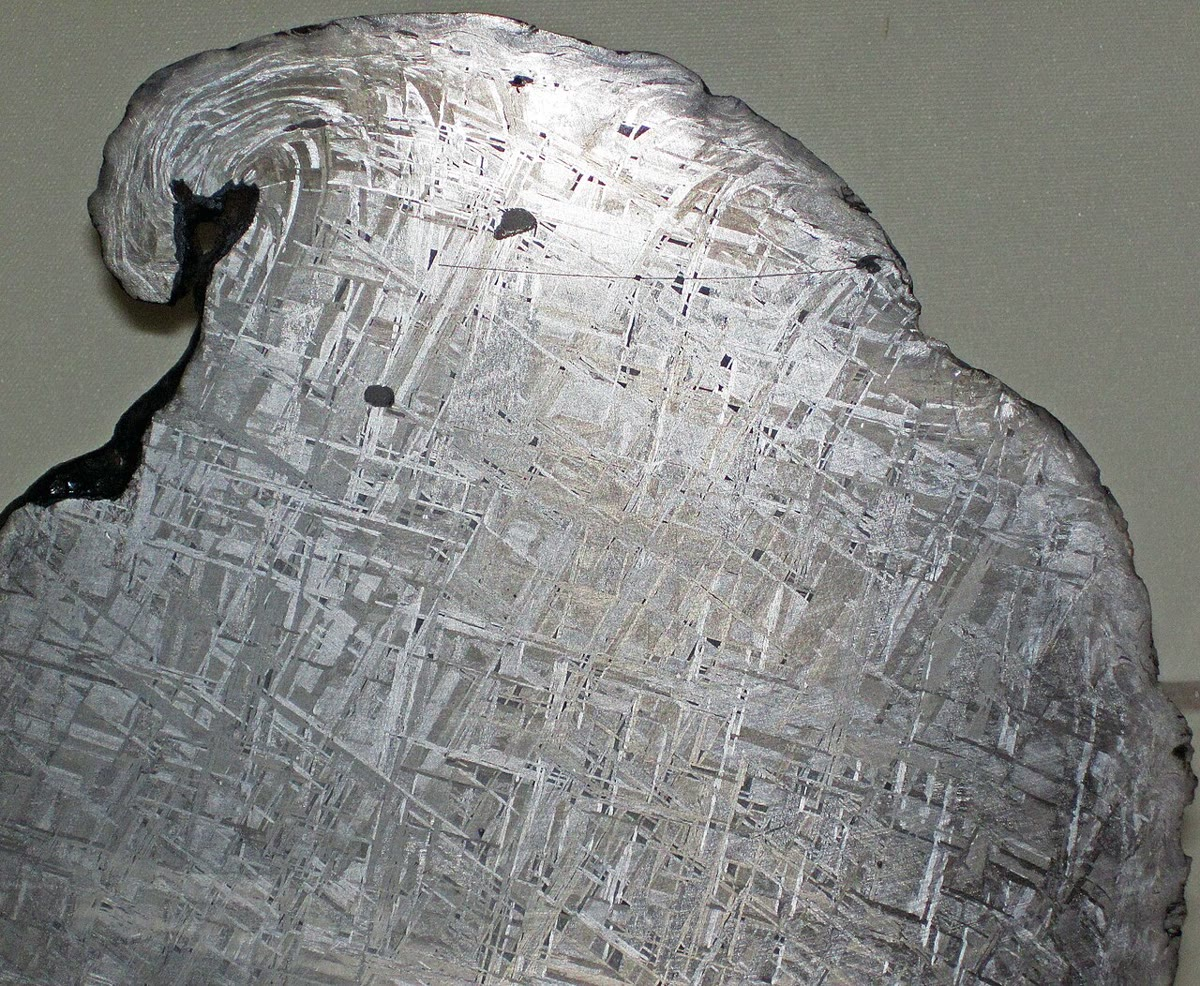
\includegraphics[width=\linewidth]{images/book4/b2-gibeon-widmanstatten.jpg}
\end{minipage}\hfill
\begin{minipage}[c]{0.46\linewidth}
{\small الوجه المقطوع والمصقول والمحفور بالحمض لقطعة من نيزك جيبيون الحديدي،
الذي عُثر عليه في ناميبيا: نمت الشبكة المتقاطعة من صفائح سبيكة الحديد والنيكل (نمط
فيدمانشتيتن) بينما كانت النواة الفلزية لجسمه الأم تبرد ببطء. James St.\ John,
CC BY 2.0.}
\end{minipage}
% ledger: data:b4-meteorites
\end{omfigure}

\section{تأريخ المجموعة الشمسية}

عمر المجموعة الشمسية هو عمر أقدم موادها الصلبة. فخطوط التساوي الزمني
لليورانيوم والرصاص في الدخائل CAI، المبنية كما في مجلد السنة الأولى، تعطي \qtyrange{4567}{4568}{\Ma}؛
وقد تكوّنت الدخائل CAI في غضون نحو \qty{0.1}{Myr} بعضها من بعض، وهو زمن قصير
بما يكفي لاعتبار عمرها لحظة ولادة الشمس. أمّا أحداث
ملايين السنين القليلة التالية، أي تكوّن \omterm{def:b2:planet-formation-meteorites:chondrule}{الكوندرولات} وتجمّع
الأجسام الأولى وانصهارها، فأفضل ما تؤرَّخ به هو نسبتها إلى الدخائل CAI، بساعات
سارت سريعًا وتوقّفت مبكرًا.
% ledger: lugaro:cai

\begin{definition}[النويدة المشعة قصيرة العمر]
\label{def:b2:planet-formation-meteorites:slr}
\emph{النويدة المشعة قصيرة العمر}\index{النويدة المشعة قصيرة العمر}
نويدة مشعة عمر نصفها من \num{0.1} إلى \qty{100}{Myr} تقريبًا،
كانت موجودة حين تكوّنت المجموعة الشمسية وهي الآن منقرضة، ويدلّ على وجودها السابق
فائضٌ من وليدتها في معادن كانت غنية
بعنصرها.
\end{definition}

أشهرها الألومنيوم 26، الذي يتحلّل إلى المغنيسيوم 26 بعمر نصف قدره
\qty{0.717}{Myr} (ومتوسط عمر قدره \qty{1.035}{Myr}). فحين تكوّنت الدخائل CAI كانت ذرّة
ألومنيوم واحدة من كل نحو \num{19000} ذرّة من الألومنيوم 26: فكانت النسبة
$\ce{^{26}Al}/\ce{^{27}Al}$ تساوي $(5.23 \pm 0.13)\times10^{-5}$، وهي القيمة
\emph{القانونية}. وتغطّي نويدات أخرى قصيرة العمر مددًا أطول (الجدول
أدناه).
% ledger: lugaro:al26, lugaro:slr-table

\begin{table}[h]
\centering
\small
\begin{tabular}{lllcc}
\hline
النويدة & الوليدة & المرجع & عمر النصف (Myr) & النسبة المبكرة\\
\hline
\ce{^{26}Al} & \ce{^{26}Mg} & \ce{^{27}Al} & 0.717 & $5.23\times10^{-5}$\\
\ce{^{60}Fe} & \ce{^{60}Ni} & \ce{^{56}Fe} & 2.62 & $1.0\times10^{-8}$\\
\ce{^{53}Mn} & \ce{^{53}Cr} & \ce{^{55}Mn} & 3.74 & $7\times10^{-6}$\\
\ce{^{107}Pd} & \ce{^{107}Ag} & \ce{^{108}Pd} & 6.5 & $6.6\times10^{-5}$\\
\ce{^{182}Hf} & \ce{^{182}W} & \ce{^{180}Hf} & 8.90 & $1.02\times10^{-4}$\\
\ce{^{129}I} & \ce{^{129}Xe} & \ce{^{127}I} & 15.7 & $1.28\times10^{-4}$\\
\hline
\end{tabular}
\caption{بعض \omterm{def:b2:planet-formation-meteorites:slr}{النويدات المشعة قصيرة العمر} في المجموعة الشمسية المبكرة، ووليدتها
المستقرة، والنظير المستقر من العنصر نفسه المستعمل مرجعًا، وعمر نصفها
ونسبتها إلى المرجع حين تكوّنت الدخائل CAI. البيانات: لوغارو
وآخرون (2018).}
\label{tab:b2:planet-formation-meteorites:slr}
% ledger: lugaro:al26, lugaro:slr-table
\end{table}

\begin{proposition}[العمر النسبي من نويدة منقرضة]
\label{prop:b2:planet-formation-meteorites:relative-age}
إذا كانت نسبة نويدة قصيرة العمر إلى نظيرها المرجعي $R_0$
في كل مكان حين تكوّنت الدخائل CAI، ووُجد أنها كانت $R$ في جسم حين
تكوّن، فإن الجسم قد تكوّن
\[
  \Delta t = \tau \ln\frac{R_0}{R}
\]
بعد الدخائل CAI، حيث $\tau$ متوسط عمر النويدة. ويعطي خطأ
$\delta R$ في $R$ الخطأ $\tau\,\delta R/R$ في $\Delta t$.
\end{proposition}

\begin{proof}
النظير المرجعي مستقر، فتتناقص النسبة كما تتناقص النويدة المشعة
نفسها: $R = R_0 e^{-\Delta t/\tau}$. وبأخذ اللوغاريتم،
$\Delta t = \tau\ln(R_0/R)$. وبالمفاضلة، $\mathrm d(\Delta t) =
-\tau\,\mathrm dR/R$.
\end{proof}

فالخطأ النسبي البالغ \qty{10}{\percent} في النسبة يكلّف إذن
\qty{0.1}{Myr} مع الألومنيوم 26، لكنه يكلّف \qty{0.54}{Myr} مع المنغنيز 53
و\qty{1.3}{Myr} مع الهافنيوم 182: فكل ساعة دقيقة على بضعة أضعاف
متوسط عمرها فقط، والساعة المناسبة تتوقّف على الحدث. وتُقرأ النسبة $R$ في
جسمٍ من معادنه.
% ledger: lugaro:al26, lugaro:slr-table

\begin{proposition}[خط التساوي الزمني للألومنيوم والمغنيسيوم]
\label{prop:b2:planet-formation-meteorites:al-mg}
لتتكوّن عدة معادن من جسم واحد معًا في الزمن $\Delta t$ بالتركيب
النظائري نفسه للمغنيسيوم، $(\ce{^{26}Mg}/\ce{^{24}Mg})_0$، لكن
بنسب $\ce{^{27}Al}/\ce{^{24}Mg}$ مختلفة، ولتبقَ مغلقة منذ ذلك الحين. فهي اليوم
تقع على المستقيم
\[
  \frac{\ce{^{26}Mg}}{\ce{^{24}Mg}}
  = \left(\frac{\ce{^{26}Mg}}{\ce{^{24}Mg}}\right)_0
  + R\,\frac{\ce{^{27}Al}}{\ce{^{24}Mg}},
\]
الذي ميله هو النسبة $R = \ce{^{26}Al}/\ce{^{27}Al}$ للجسم حين
تكوّنه.
\end{proposition}

\begin{proof}
كل ذرّة ألومنيوم 26 كانت موجودة عند التكوّن صارت منذ ذلك الحين
ذرّة مغنيسيوم 26، فاكتسب المعدن
$\ce{^{26}Al}_{\text{آنذاك}} = R\,\ce{^{27}Al}$ ذرّة من المغنيسيوم 26، إذ إن الألومنيوم 27
مستقر. وبالقسمة على عدد ذرّات المغنيسيوم 24، الذي لم يتغيّر،
نحصل على المستقيم.
\end{proof}

تُظهر المعادن الغنية بالألومنيوم والفقيرة بالمغنيسيوم، مثل البلاجيوكلاز، فوائض كبيرة
من المغنيسيوم 26؛ أمّا الأوليفين، الخالي تقريبًا من الألومنيوم، فلا يُظهر شيئًا منها. وهكذا
بُني التسلسل الزمني للمجموعة الشمسية المبكرة: الدخائل CAI أولًا؛ ثم \omterm{def:b2:planet-formation-meteorites:chondrule}{الكوندرولات} على مدى
ملايين السنين القليلة التالية، وتحدّد الأدلةُ المستقاة من \omterm{def:b2:planet-formation-meteorites:chondrule}{الكوندرولات}
عمرَ القرص الغازي بأقل من خمسة ملايين سنة؛ ثم تجمّعت الأجسام الأم
للكوندريتات بعد أحدث كوندرولاتها. وقد بدأت الديوجينايتات،
وهي صخور وشاح فيستا، تتبلّر في غضون نحو مليون سنة من
الدخائل CAI، وتكوّنت نواة فيستا في غضون السنوات الأولى من مليون إلى
أربعة ملايين: \omterm{def:b2:planet-formation-meteorites:classes}{فالنيازك الحديدية} \omterm{def:b2:planet-formation-meteorites:classes}{والأكوندريتات} أقدم من كثير من
الكوندريتات.
% ledger: lugaro:cai, gail:vesta, gail:meteorites

\section{حرارة الألومنيوم 26 والانصهار الأول}

من أين جاءت الحرارة التي صهرت فيستا وحوّلت الكوندريتات
العادية؟ تتّفق النماذج والنيازك على أن المصدر الغالب في أقدم الأجسام
كان تحلّل الألومنيوم 26. ففي صخر ذي تركيب كوندريتي كان يحمل، في البداية،
\qty{5}{MJ} لكل كيلوغرام جاهزة للتحرّر في غضون بضعة ملايين من السنين:
وهذا يكفي لتسخين الصخر آلاف الكلفنات، لو لم تستطع الحرارة الإفلات.
% ledger: lugaro:heat, lugaro:melting

\begin{proposition}[تسخين كويكب بدائي بالألومنيوم 26]
\label{prop:b2:planet-formation-meteorites:heating}
الصخر الذي يتلقّى القدرة الإشعاعية $H_0 e^{-t/\tau}$ لكل كيلوغرام، وسعته
الحرارية النوعية $c$، ولا يفقد حرارة، يسخن بعد تراكمه في
الزمن $t_a$ وفق
\[
  T(t) = T_0 + \frac{H_0\tau}{c}\left(e^{-t_a/\tau} - e^{-t/\tau}\right),
\]
ويؤول إلى درجة حرارة الذروة
$T_{\max} = T_0 + (H_0\tau/c)\,e^{-t_a/\tau}$. ولا تُبلغ درجة حرارة حرجة
$T_c > T_0$ إلا إذا تراكم الجسم قبل
\[
  t_a^* = \tau\ln\frac{H_0\tau}{c\,(T_c - T_0)}.
\]
\end{proposition}

\begin{proof}
مع انعدام الفقد، $c\,\mathrm dT/\mathrm dt = H_0 e^{-t/\tau}$. وبالتكامل ابتداءً من
$t_a$، حيث $T = T_0$، نحصل على
$c\,(T - T_0) = H_0\tau\,(e^{-t_a/\tau} - e^{-t/\tau})$، الذي يؤول إلى
$H_0\tau e^{-t_a/\tau}$ عندما $t \to \infty$. وبوضع $T_{\max} = T_c$ والحلّ
بالنسبة إلى $t_a$ نحصل على $t_a^*$؛ ومع تراكم أبكر تكون الذروة أعلى.
\end{proof}

يستعمل نموذجٌ للجسم الأم للكوندريتات العادية
$H_0 = \qty{1.9e-7}{W.kg^{-1}}$ و$c = \qty{837}{J.kg^{-1}.K^{-1}}$
و$T_0 = \qty{250}{K}$. فتكون $H_0\tau/c$ نحو \qty{7400}{K}. وثلاث
درجات حرارة مهمة: قرب \qty{750}{K} يبدأ الصخر المسامي بالتلبّد ليصير
صخرًا متراصًّا؛ وقرب \qty{1200}{K} يبدأ الفلز وكبريتيد الحديد بالانصهار
معًا؛ وقرب \qty{1700}{K} تنصهر آخر السيليكات. فالجسم الذي تراكم
قبل \qty{1.7}{Myr} انصهر كليًّا؛ وقبل \qty{2.1}{Myr} انصهر فلزه وكبريتيده
واستطاعا الغوص ليكوّنا نواة؛ وحتى نحو \qty{2.8}{Myr} كان على الأقل
متلبّدًا ومتحوّلًا؛ أمّا الأجسام اللاحقة فبقيت باردة (الشكل أدناه).
% ledger: gail:params, gail:temps, lugaro:al26

\begin{omfigure}
\begin{tikzpicture}
\begin{axis}[omrecord, name=left, width=0.45\linewidth, height=6.0cm,
  xmin=0, xmax=8, ymin=0, ymax=2300,
  xlabel={الزمن بعد الدخائل \babelsublr{CAI} \babelsublr{(Myr)}}, ylabel={درجة الحرارة \babelsublr{(\unit{K})}},
  tick label style={font=\scriptsize}, label style={font=\small}]
\addplot[black!45, densely dashed, domain=0:8, samples=2] {750};
\addplot[black!45, densely dashed, domain=0:8, samples=2] {1200};
\addplot[black!45, densely dashed, domain=0:8, samples=2] {1700};
\addplot[thick, red!75!black] table[x=t_Myr, y=T_K] {figdata/out/bachelor-2-al26-ta15.dat};
\addplot[thick, orange!80!black] table[x=t_Myr, y=T_K] {figdata/out/bachelor-2-al26-ta20.dat};
\addplot[thick, teal!70!black] table[x=t_Myr, y=T_K] {figdata/out/bachelor-2-al26-ta25.dat};
\addplot[thick, blue!70!black] table[x=t_Myr, y=T_K] {figdata/out/bachelor-2-al26-ta30.dat};
\node[font=\tiny, red!75!black, anchor=south east] at (axis cs:7.9,1995) {$t_a = \qty{1.5}{Myr}$};
\node[font=\tiny, orange!80!black, anchor=south east] at (axis cs:7.9,1325) {2};
\node[font=\tiny, teal!70!black, anchor=south east] at (axis cs:7.9,915) {2.5};
\node[font=\tiny, blue!70!black, anchor=north east] at (axis cs:7.9,650) {3};
\node[font=\tiny, black!60, anchor=south west] at (axis cs:0.1,1700) {انصهار السيليكات};
\node[font=\tiny, black!60, anchor=south west] at (axis cs:0.1,1200) {انصهار Fe وFeS};
\node[font=\tiny, black!60, anchor=south west] at (axis cs:0.1,750) {التلبّد};
\end{axis}
\begin{axis}[omrecord, at={(left.east)}, anchor=west, xshift=2.1cm, width=0.45\linewidth,
  height=6.0cm, xmin=0, xmax=4, ymin=0, ymax=8000,
  xlabel={زمن التراكم $t_a$ \babelsublr{(Myr)}}, ylabel={درجة حرارة الذروة \babelsublr{(\unit{K})}},
  tick label style={font=\scriptsize}, label style={font=\small},
  scaled y ticks=false, yticklabel style={/pgf/number format/1000 sep={\,}}]
\addplot[black!45, densely dashed, domain=0:4, samples=2] {750};
\addplot[black!45, densely dashed, domain=0:4, samples=2] {1200};
\addplot[black!45, densely dashed, domain=0:4, samples=2] {1700};
\addplot[thick, black] table[x=ta_Myr, y=Tpeak_K] {figdata/out/bachelor-2-al26-peak.dat};
\draw[black!60] (axis cs:1.69,0) -- (axis cs:1.69,1700);
\draw[black!60] (axis cs:2.13,0) -- (axis cs:2.13,1200);
\node[font=\tiny, black!70, anchor=south] at (axis cs:2.0,4500) {\qty{1.7}{Myr}};
\draw[black!50, -latex] (axis cs:2.0,4450) -- (axis cs:1.71,1800);
\node[font=\tiny, black!70, anchor=south] at (axis cs:2.9,3300) {\qty{2.1}{Myr}};
\draw[black!50, -latex] (axis cs:2.9,3250) -- (axis cs:2.16,1300);
\end{axis}
\end{tikzpicture}

\par\smallskip{\small تسخين داخل جسم كوندريتي بالألومنيوم 26 دون
فقد للحرارة (القضية أعلاه؛ $H_0 = \qty{1.9e-7}{W.kg^{-1}}$،
$c = \qty{837}{J.kg^{-1}.K^{-1}}$، $T_0 = \qty{250}{K}$، $\tau = \qty{1.035}{Myr}$).
يسارًا: درجة الحرارة بدلالة الزمن لأجسام تراكمت بعد 1.5 و2 و2.5 و\qty{3}{Myr}
من الدخائل CAI. يمينًا: درجة حرارة الذروة بدلالة زمن التراكم؛ فالأجسام التي تراكمت
قبل \qty{1.7}{Myr} انصهرت، والتي تراكمت قبل \qty{2.1}{Myr} انصهر فلزها وكبريتيدها.
وتنفق الأجسام الحقيقية جزءًا من الحرارة على الانصهار، مما يحدّ درجة الحرارة، وتفقد
حرارة قرب سطحها. قيم النموذج: غيل وآخرون (2014).}
% ledger: gail:params, gail:temps, lugaro:al26
\end{omfigure}

تُهمل القضية فقد الحرارة، وهذا لا يصحّ إلا في أعماق جسم كبير.
فالحرارة تنتشر على المسافة $\sqrt{\kappa t}$ في الزمن $t$، حيث
$\kappa$ الانتشارية الحرارية للصخر: ومع قيم النموذج يكون ذلك
نحو \qty{5}{km} في متوسط عمر واحد للألومنيوم 26 (\cref{exo:b2:planet-formation-meteorites:12}). والأجسام الأصغر
من ذلك بكثير تفقد حرارتها بالسرعة التي تنتجها بها؛ وتبيّن النماذج التفصيلية
أن الأجسام التي يزيد قطرها على 10 إلى \qty{20}{km} أمكنها أن تنصهر.
% ledger: gail:params, lugaro:melting

\begin{definition}[التمايز الكوكبي]
\label{def:b2:planet-formation-meteorites:differentiation}
\emph{التمايز الكوكبي}\index{التمايز الكوكبي} هو
انفصال جسم، منصهر أو منصهر جزئيًا، إلى طبقات مختلفة
التركيب والكثافة: نواة فلزية، ووشاح سيليكاتي، وقشرة مكوّنة من
آخر المصاهير.
\end{definition}

تسجّل النيازك إذن نوعين من الأجسام المبكرة. فالتي تكوّنت في غضون
نحو المليونَي سنة الأوليين كان لديها من الألومنيوم 26 ما يكفي لتنصهر
وتتمايز: فنواها هي \omterm{def:b2:planet-formation-meteorites:classes}{النيازك الحديدية}، وقشورها ووشاحاتها
\omterm{def:b2:planet-formation-meteorites:classes}{الأكوندريتات}، وفيستا هو الناجي منها. أمّا التي تكوّنت لاحقًا فبقيت
كوندريتات، سُخّنت من الداخل بدرجة حدّدها تاريخ ولادتها
وعمق كل شظية: فصار الأعمق من النمط 6، وبقي الأقرب إلى السطح
من النمط 3. والأرض نفسها، المبنية من أجنّة \omterm{def:b2:planet-formation-meteorites:planetesimal}{وكويكبات بدائية} من النوعين
والمضروبة بتصادمات عملاقة، تمايزت إلى نواتها ووشاحها وقشرتها.
% ledger: gail:meteorites, gail:vesta, gail:temps

\section{التمارين}

\begin{exercise}[$\star$]\label{exo:b2:planet-formation-meteorites:1}
في \omterm{def:b2:planet-formation-meteorites:nebula}{السديم الشمسي} ذي الكتلة الدنيا، احسب الكثافة السطحية للغاز عند
\qty{1}{au} وعند \qty{5.2}{au}، والكثافة السطحية للمواد الصلبة عند
\qty{1}{au} (الصخر وحده، $Z_{\mathrm{rel}} = 0.33$) وعند \qty{5.2}{au} (كل أنواع الجليد
متكاثفة، $Z_{\mathrm{rel}} = 1$). كم مرة يفوق الغاز المواد الصلبة كتلةً
عند \qty{5.2}{au}؟
% ledger: cy10:mmsn
\end{exercise}

\begin{exercise}[$\star$]\label{exo:b2:planet-formation-meteorites:2}
مستعينًا بشكل درجات حرارة التكاثف، رتّب الألومنيوم والصوديوم
والمغنيسيوم والحديد والكبريت والأكسجين (في صورة جليد الماء) من أوّلها تكاثفًا إلى
آخرها، واذكر مجموعة التطاير لكل منها. أيّها تتوقّع
أن تجده غنيًا في الدخائل CAI، وأيّها فقيرًا في الأرض مقارنةً بالشمس؟
% ledger: lodders:tc-table, lodders:groups
\end{exercise}

\begin{exercise}[$\star$]\label{exo:b2:planet-formation-meteorites:3}
يذكر الفهرس \num{1107} سقطات، منها 856 كوندريتًا عاديًا
و49 نيزكًا حديديًا، و\num{44534} لقية، منها \num{38647} كوندريتًا عاديًا
و\num{1020} نيزكًا حديديًا و\num{22096} آتية من جنوب \ang{60}\,ج. احسب
حصّة الكوندريتات العادية \omterm{def:b2:planet-formation-meteorites:classes}{والنيازك الحديدية} بين السقطات وبين اللقيات،
وحصّة لقيات القارة القطبية الجنوبية. أيّ العيّنتين تستعمل لتقدير
النسب التي تصل بها الأصناف إلى الأرض، ولماذا؟
% ledger: data:b4-meteorites
\end{exercise}

\begin{exercise}[$\star$]\label{exo:b2:planet-formation-meteorites:4}
تعطي معادن جسمٍ النسبةَ الابتدائية
$\ce{^{26}Al}/\ce{^{27}Al} = \num{1.0e-5}$. بعد كم من الزمن من الدخائل CAI تكوّن؟
خذ $R_0 = \num{5.23e-5}$ ومتوسط عمر قدره \qty{1.035}{Myr}.
% ledger: lugaro:al26
\end{exercise}

\begin{exercise}[$\star\star$]\label{exo:b2:planet-formation-meteorites:5}
باستعمال \cref{prop:b2:planet-formation-meteorites:disc-mass} مع
$\Sigma_1 = \qty{2.2e4}{kg.m^{-2}}$ عند \qty{1}{au} (\qty{1}{au} $=
\qty{1.496e11}{m}$، $M_\odot = \qty{1.989e30}{kg}$)، احسب كتلة
السديم ذي الكتلة الدنيا داخل \qty{30}{au} وداخل \qty{100}{au}، بالكتل
الشمسية. وقارن بالأقراص المرصودة، من 0.001 إلى 0.1 كتلة شمسية.
% ledger: cy10:mmsn
\end{exercise}

\begin{exercise}[$\star\star$]\label{exo:b2:planet-formation-meteorites:6}
في القرص السلبي $T = \qty{120}{K}\,(r/\qty{1}{au})^{-3/7}$، أوجد أين يصير جليد
الماء (\qty{182}{K}) وجليد الميثان (\qty{41}{K}) مستقرّين. والحبيبة المعرّضة لضوء الشمس
المباشر تبلغ \qty{182}{K} عند \qty{2.3}{au}. لماذا يختلف التقديران \omterm{def:b2:planet-formation-meteorites:snow-line}{لخط
الثلج}، وأيّهما ينطبق على الأجسام التي بنت الكواكب؟
% ledger: cy10:passive, lodders:phases
\end{exercise}

\begin{exercise}[$\star\star$]\label{exo:b2:planet-formation-meteorites:7}
احسب كتلة العزلة، مع $b = 5$، لجنين عند \qty{1}{au} في
السديم ذي الكتلة الدنيا ($\Sigma_p = \qty{10.9}{g.cm^{-2}}$)، وعند \qty{5.2}{au}
وراء \omterm{def:b2:planet-formation-meteorites:snow-line}{خط الثلج} ($\Sigma_p = \qty{2.78}{g.cm^{-2}}$)، بالكتل الأرضية
($M_\oplus = \qty{5.972e24}{kg}$، $M_\odot = \qty{1.989e30}{kg}$). وكم تصير
عند \qty{5.2}{au} في قرص فيه من المواد الصلبة \num{3.5} أضعاف؟
% ledger: cy10:isolation, cy10:mmsn, earth:mass
\end{exercise}

\begin{exercise}[$\star\star$]\label{exo:b2:planet-formation-meteorites:8}
كان صخر ذو تركيب CI يحوي \num{1.01e16} ذرّة من الألومنيوم 26 في الغرام حين
تكوّنت الدخائل CAI، وكل تحلّل يترك \qty{5.00e-13}{J} من الحرارة. احسب
الحرارة المتحرّرة لكل كيلوغرام على مدى التحلّل كله، والارتفاع في درجة الحرارة الذي
تعطيه مع $c = \qty{837}{J.kg^{-1}.K^{-1}}$ ودون فقد. كم مرة
تفوق الحرارةَ اللازمة لتسخين الصخر من \num{250} إلى
\qty{1700}{K}؟
% ledger: lugaro:heat, gail:params
\end{exercise}

\begin{exercise}[$\star\star$]\label{exo:b2:planet-formation-meteorites:9}
على مدى تحلّله كله، يحرّر الألومنيوم 26 \qty{5.07e10}{erg} لكل غرام من صخر CI،
ويحرّر الحديد 60 \qty{7.49e7}{erg} لكل غرام. احسب نسبة
الطاقتين. وعمر نصف الحديد 60 هو \qty{2.62}{Myr}: احسب متوسط عمره،
ونسبة قدرتي التسخين الابتدائيتين، أي الطاقة مقسومة على متوسط العمر.
% ledger: lugaro:heat, lugaro:slr-table, lugaro:al26
\end{exercise}

\begin{exercise}[$\star\star\star$]\label{exo:b2:planet-formation-meteorites:10}
مستعينًا بنتائج \cref{exo:b2:planet-formation-meteorites:9}، أوجد الزمن الذي يصير بعده الحديد 60 يسخّن الصخر
أسرع من الألومنيوم 26. هل كان الحديد 60 قادرًا على صهر جسم تراكم في هذا الوقت
المتأخر؟ (قارن الطاقة التي لا يزال عليه أن يحرّرها حينئذ بالمقدار
\qty{1.2e6}{J.kg^{-1}} اللازم لتسخين الصخر من \num{250} إلى \qty{1700}{K}.)
% ledger: lugaro:heat, lugaro:slr-table, lugaro:al26
\end{exercise}

\begin{exercise}[$\star\star\star$]\label{exo:b2:planet-formation-meteorites:11}
مع $H_0 = \qty{1.9e-7}{W.kg^{-1}}$ و$\tau = \qty{1.035}{Myr}$
و$c = \qty{837}{J.kg^{-1}.K^{-1}}$ و$T_0 = \qty{250}{K}$ (السنة
\qty{3.156e7}{s})، احسب أبعد زمنَي تراكم يبلغ فيهما مركز
جسم كبير \qty{1200}{K} و\qty{1700}{K}. تشير بعض القياسات إلى أن
الألومنيوم 26 الابتدائي لم يكن إلا نصف القيمة القانونية في أجزاء من القرص:
فبكم ينزاح الزمنان؟ بيّن أن الانزياح لا يتوقّف على
درجة الحرارة الحرجة.
% ledger: gail:params, gail:temps, lugaro:al26
\end{exercise}

\begin{exercise}[$\star\star\star$]\label{exo:b2:planet-formation-meteorites:12}
لصخرٍ موصليته \qty{2.1}{W.m^{-1}.K^{-1}}، وكثافته
\qty{3300}{kg.m^{-3}}، وسعته الحرارية النوعية \qty{837}{J.kg^{-1}.K^{-1}}،
انتشاريةٌ حرارية $\kappa = k/(\rho c)$. احسبها، واحسب المسافة
$\sqrt{\kappa\tau}$ التي تنتشر عليها الحرارة في متوسط عمر واحد للألومنيوم 26.
اشرح لماذا تنطبق قضية التسخين على مركز جسم قطره
\qty{100}{km} ولا تنطبق على جسم قطره \qty{2}{km}، وقارن بأصغر
الأجسام التي أمكنها الانصهار، وقطرها من 10 إلى \qty{20}{km}.
% ledger: gail:params, lugaro:melting, lugaro:al26
\end{exercise}

\section{مسألة: الحجر الذي سقط على البحيرة المتجمّدة}

\begin{problem}[{مسألة نهاية الأسبوع --- تصنيف حجر سقط حديثًا، وتأريخ
كوندرولاته بالألومنيوم 26، ومعرفة الدرجة التي بلغتها حرارة جسمه الأم}]
\label{pb:b2:planet-formation-meteorites:1}
% values: calc/ch02.py
% ledger: data:b4-meteorites, gail:chondrite-table, lugaro:al26, lugaro:cai, gail:params, gail:temps, cy10:mmsn, cy10:isolation, lodders:tc-table, earth:mass
في ليلة شتوية تعبر كرةٌ نارية السماءَ فوق بحيرة شمالية متخيَّلة،
ويُسمع دويّ. وفي الصباح التالي يُلتقط من على الجليد حجر ذو قشرة سوداء كتلته \qty{2.4}{kg}،
في وسط حفرة حديثة في الثلج. ويُظهر الحجر المقطوع
كوندرولات تشغل \qty{75}{\percent} من حجمه، متوسط قطرها \qty{0.3}{mm}،
وحوافها باهتة؛ ويشغل الفلز \qty{9}{\percent} من
حجمه، ويحوي أوليفينه 18 في المئة مولية من الفاياليت. ويحلّل مختبرٌ
كوندرولًا واحدًا (الجدول أدناه). استعمل جداول الفصل،
و$R_0 = \num{5.23e-5}$، و$\tau = \qty{1.035}{Myr}$، والسنة \qty{3.156e7}{s}،
و$H_0 = \qty{1.9e-7}{W.kg^{-1}}$، و$c = \qty{837}{J.kg^{-1}.K^{-1}}$،
و$T_0 = \qty{250}{K}$، وموصلية قدرها \qty{2.1}{W.m^{-1}.K^{-1}}، وكثافة قدرها
\qty{3300}{kg.m^{-3}}، و\qty{1}{au} $= \qty{1.496e11}{m}$،
و$M_\odot = \qty{1.989e30}{kg}$ و$M_\oplus = \qty{5.972e24}{kg}$.

\begin{center}
\small
\begin{tabular}{lcc}
\hline
المعدن & $\ce{^{27}Al}/\ce{^{24}Mg}$ & $\ce{^{26}Mg}/\ce{^{24}Mg}$\\
\hline
الأوليفين & 0.05 & \num{0.139500}\\
الزجاج & 3.00 & \num{0.139518}\\
البلاجيوكلاز & 15.0 & \num{0.139590}\\
\hline
\end{tabular}
\end{center}

\medskip
\noindent\textbf{الجزء الأول --- الحجر.}
\begin{enumerate}
  \item هل الحجر سقطة أم لقية؟ ولماذا يجعله ذلك ثمينًا؟
  \item من بين سقطات الفهرس البالغة \num{1107}، هناك 856 كوندريتًا عاديًا. ما
        احتمال أن تكون سقطة مأخوذة عشوائيًا واحدًا منها؟
  \item مستعينًا بجدول مجموعات الكوندريتات، اذكر المجموعة التي ينتمي إليها الحجر.
  \item حواف كوندرولاته باهتة ومعادنه متجانسة
        التركيب. ما \omterm{def:b2:planet-formation-meteorites:type}{الأنماط الصخرية} التي يوحي بها ذلك، وما
        أعلى درجة حرارة بلغتها مجموعته، بالكلفن وبالدرجات المئوية؟
  \item لماذا تتوقّع أن تجد فيه قليلًا من الدخائل CAI، ولماذا يبقى الحجر مع ذلك
        أحدث من أي دخيلة CAI؟
\end{enumerate}

\noindent\textbf{الجزء الثاني --- متى تكوّن \omterm{def:b2:planet-formation-meteorites:chondrule}{الكوندرول}؟}
\begin{enumerate}[resume]
  \item اشرح لماذا ترتفع النسبة $\ce{^{26}Mg}/\ce{^{24}Mg}$ مع
        $\ce{^{27}Al}/\ce{^{24}Mg}$ من معدن إلى آخر.
  \item من الأوليفين والبلاجيوكلاز، احسب ميل خط التساوي الزمني.
        ماذا يقيس؟
  \item تحقّق من أن الزجاج يقع على المستقيم نفسه.
  \item بعد كم من الزمن من الدخائل CAI تكوّن \omterm{def:b2:planet-formation-meteorites:chondrule}{الكوندرول}؟
  \item باعتبار عمر الدخائل CAI \qty{4567.5}{\Ma}، أعطِ عمر \omterm{def:b2:planet-formation-meteorites:chondrule}{الكوندرول}.
  \item كم كانت النسبة $\ce{^{26}Al}/\ce{^{27}Al}$ لتكون في معدن تكوّن
        بعد \qty{10}{Myr} من الدخائل CAI؟ وأيّ نويدة من الجدول تؤرّخ مثل هذا
        الحدث على نحو أفضل؟
\end{enumerate}

\noindent\textbf{الجزء الثالث --- تسخين الجسم الأم.}
تجمّع الجسم الأم للحجر، ونصف قطره \qty{20}{km}، بعد \qty{2.4}{Myr} من
الدخائل CAI، بُعيد تكوّن كوندرولاته.
\begin{enumerate}[resume]
  \item احسب الانتشارية الحرارية للصخر والزمن $R^2/\kappa$ اللازم
        لإفلات الحرارة من المركز، بملايين السنين. هل يجوز أن يُعامل المركز
        على أنه لا يفقد حرارة؟
  \item احسب قدرة التسخين للألومنيوم 26 لكل كيلوغرام من الصخر في زمن
        التجمّع.
  \item احسب الحرارة التي لا يزال يتعيّن تحريرها لكل كيلوغرام بعد التجمّع.
  \item احسب الارتفاع في درجة الحرارة ودرجة حرارة الذروة في المركز.
  \item قارن بدرجات الحرارة الحرجة الثلاث في الفصل. هل انصهر
        المركز؟ وهل يتّسق ذلك مع السؤال 4؟
  \item ما أبعد زمن تجمّع كان سيبدأ معه فلز المركز وكبريتيده
        بالانصهار؟
  \item بعد كم من الزمن من التجمّع يُبلغ \qty{90}{\percent} من الارتفاع في درجة
        الحرارة؟ أعطِ التاريخ بعد الدخائل CAI.
\end{enumerate}

\noindent\textbf{الجزء الرابع --- الجيران.}
\begin{enumerate}[resume]
  \item يأتي أكوندريت من جسم تجمّع بعد \qty{0.8}{Myr} من
        الدخائل CAI. احسب درجة حرارة الذروة التي كانت القضية لتعطيها، واذكر
        ما حدث للجسم فعلًا.
  \item كم مرة كان لدى ذلك الجسم من الألومنيوم 26 لكل كيلوغرام عند
        تجمّعه أكثر مما كان لدى الجسم الأم للحجر؟
  \item الحجر أفقر من الشمس في الزنك والرصاص، لكنه ليس أفقر منها في المغنيسيوم ولا في
        الألومنيوم. استعمل درجات حرارة التكاثف لتفسير ذلك.
  \item في السديم ذي الكتلة الدنيا، احسب الكثافة السطحية للصخر
        ($Z_{\mathrm{rel}} = 0.33$) عند \qty{2.5}{au}، حيث كان يدور الجسم
        الأم.
  \item احسب كتلة العزلة عند \qty{2.5}{au}، مع $b = 5$، بالكيلوغرام
        وبالكتل الأرضية، وقارنها بكتلة الجسم الأم.
  \item اذكر درجة حرارة الذروة في مركز الجسم الأم، وهي الرقم الأساسي
        في هذه المسألة، بالدرجات المئوية.
\end{enumerate}
\end{problem}
